\begin{enumerate}
 \item 
\begin{enumerate}
 \item 
 Après développement simplification et factorisation, on trouve
\begin{multline*}
 P(m_1,m_2,m_3,m_4)=\\ m_2m_4 - m_2m_3 - m_1m_4 + m_1m_3 + m_4m_3 - m_4m_2 - m_1m_3 + m_1m_2\\
= - m_2m_3 - m_1m_4  + m_4m_3 + m_1m_2 
= m_3(m_4 -m_2) - m_1(m_4 - m_2)\\ =(m_3-m_1)(m_4-m_2) 
\end{multline*}

\item Notons $m_1$, $m_2$, $m_3$, $m_4$ les affixes des quatre points $M_1$, $M_2$, $M_3$, $M_4$.\newline
 L'inégalité de Ptolémée est une conséquence de l'inégalité triangulaire appliquée à la relation de la question 1.a.
\end{enumerate}

 \item 
\begin{enumerate}
 \item \'Elevons au carré et développons ($a$ et $b$ sont non  nuls)
\begin{multline*}
 |a+b| = |a|+|b|\Leftrightarrow |a|^2 + |b|^2 +2\Re(a\,\overline{b}) = |a|^2 + |b|^2 +2|a||b|\\
\Leftrightarrow \Re(a\,\overline{b}) = |a||b| \Leftrightarrow \Re(\frac{a}{b})= \left\vert \frac{a}{b}\right\vert
\end{multline*}
 Si un nombre complexe est un réel strictement positif, il est égal à son module. Réciproquement, si $\Re(z) = |z|$ alors $\Im(z)=0$ donc $z=\Re(z)$ et $z\in \R_+^*$.
 \item L'égalité dans l'inégalité de Ptolémée est équivalente à l'égalité dans l'inégalité triangulaire. D'après le a. elle est équivalente à (configuration d'égalité)
\begin{displaymath}
 B(m_1,m_2,m_3,m_4) \in \R_+^*
\end{displaymath}

 \item Considérons une similitude $S$ quelconque. Il existe alors des complexes $a$ et $b$ avec $a\neq0$ tel que, pour tout $M$ d'affixe $m$, l'affixe de $S(M)$ est $az+b$. Notons la $s(m)$. Dans l'expression de $s(m_i)-s(m_j)$, les $b$ se simplifie et les $a$ se factorisent. Ils se simplifient dans l'exprssion complète du birapport qui est donc conservé.
\begin{displaymath}
 B(s(m_1),s(m_2),s(m_3),s(m_4))= B(m_1,m_2,m_3,m_4)
\end{displaymath}
 On en déduit que si $(M_1,M_2,M_3,M_4)$ est une configuration d'égalité alors $(S(M_1),S(M_2),S(M_3),S(M_4))$ est encore une configuration d'égalité.
\end{enumerate}

 \item On suppose que $M_1$, $M_2$, $M_3$, $M_4$ sont dans cet ordre sur une même droite. Il existe alors un nombre complexe $a$ (affixe d'un point de la droite), un nombre complexe non nul $u$ (affixe d'un vecteur directeur de la droite) et des réels $\lambda_1$, $\lambda_2$, $\lambda_3$, $\lambda_4$ tels que
\begin{displaymath}
 m_1=a+\lambda_1u,m_2=a+\lambda_2u, m_3=a+\lambda_3u, m_4=a+\lambda_4u \text{ avec }
\lambda_1 < \lambda_2 < \lambda_3 < \lambda_4  
\end{displaymath}
La famille est alors dans une configuration d'égalité car:
\begin{displaymath}
 B(m_1,m_2,m_3,m_4) = B(\lambda_1,\lambda_2,\lambda_3,\lambda_4)\in \R_+^*
\end{displaymath}

 \item 
\begin{enumerate}
 \item Dans cette question, on exprime systématique chaque différence de deux exponentielles par la formule suivante:
\begin{displaymath}
 e^{i\alpha}-e^{i\beta} = 2i\sin(\frac{\alpha - \beta}{2})e^{i\frac{\alpha + \beta}{2}}
\end{displaymath}
Dans l'expression de $B$, les $2i$ et les exponentielles de simplifient. Il reste
\begin{displaymath}
 B(m_1,m_2,m_3,m_4)=\frac{\sin\left(\frac{\alpha_2 - \alpha_1}{2}\right) \sin\left(\frac{\alpha_4 - \alpha_3}{2}\right)}
                         {\sin\left(\frac{\alpha_4 - \alpha_1}{2}\right) \sin\left(\frac{\alpha_3 - \alpha_2}{2}\right)}
\end{displaymath}
 
 \item Lorsque les points $M_1$, $M_2$, $M_3$, $M_4$ sont sur le cercle unité et dans cet ordre pour le sens trigonométrique, il n'existe pas forcément d'arguments tels que $0\leq \alpha_1 < \alpha_2 < \alpha_3 < \alpha_4 < 2\pi$. En revanche il existe des arguments tels que les différences vérifient
\begin{displaymath}
  0< \alpha_2 - \alpha_1 < \alpha_3 - \alpha_1 < \alpha_4 - \alpha_1 < 2\pi
\end{displaymath}
\begin{figure}
 \centering
 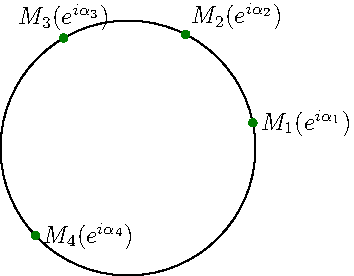
\includegraphics{./Cptolem_1.pdf}
 % Cptolem_1.pdf: 0x0 pixel, 0dpi, 0.00x0.00 cm, bb=
  \caption{Une configuration d'égalité (question \theenumi.\theenumii) }
 \label{fig:Cptolem_1}
\end{figure}

On en déduit que tous les $\alpha_i - \alpha_j$ sont dans $]0,2\pi[$ donc, dans l'expression de $B$, tous les arguments des $\sin$ sont dans $]0,\pi[$. Les $\sin$ sont donc tous strictement positifs ce qui prouve que la famille de points est dans une configuration d'égalité.  
\end{enumerate}

 \item 
\begin{enumerate}
 \item En utilisant les relations données au début du problème, on obtient:
\begin{displaymath}
 B(m_1,m_2,m_3,m_4)=
\frac{\frac{1}{z_2}(\frac{1}{z_4}-\frac{1}{z_3})}{\frac{1}{z_4}(\frac{1}{z_3}-\frac{1}{z_2})}
=\frac{z_3 -z_4}{z_2-z_3}
\end{displaymath}
 
 \item D'après les questions précédentes, la famille $(M_1,M_2,M_3,M_4)$ est dans une configuration d'égalité si et seulement si 
 $\frac{z_4 -z_3}{z_2-z_3}$ est un réel strictement négatif. Cela traduit que les points $Z_2$, $Z_3$, $Z_4$ sont alignés et que $Z_3$ appartient au segment $[Z_1, Z_4]$.\newline
 On peut démontrer (voir le \href{http://maquisdoc.net/data/cours\_nicolair/C2002.pdf}{cours sur les complexes} ) que cette condition d'alignement des $Z_i$ se traduit par la cocyclicité (être sur le même cercle) des $M_i$.
\end{enumerate}

\end{enumerate}
